\documentclass[12pt,letterpaper]{article}
\usepackage[utf8]{inputenc}
\usepackage[T1]{fontenc}
\usepackage[spanish]{babel}
\usepackage{geometry}
\usepackage{graphicx}
\usepackage{algorithm}
\usepackage{algpseudocode}


\geometry{top=2.5cm, bottom=2.5cm, left=2.5cm, right=2.5cm}


\usepackage{fancyhdr}
\pagestyle{fancy}
\fancyhf{} 


\lhead{Luis Enrique Escamilla Rufina}
\rhead{FCiencias}
\cfoot{\thepage}

\renewcommand{\headrulewidth}{0.6pt} 


\title{Base de datos musical con un Minero y una Interfaz gráfica}
\author{Luis Enrique Escamilla Rufina}

\begin{document}

\maketitle
\thispagestyle{fancy} 

\section{Resumen}
El segundo proyecto de Modelado y Programación, que consiste hacer una implementacion de base de datos mediante SQLite, que tenga un minero para poder minar en directorios y encontrar archivos .mp3, los cuales se extraen los datos de su etiqueta ID3v2.4.0 para poder llenar con esto la Base de datos. Además de tener una interfaz gráfica con la que se permita minar los directorios y presentar la tabla con las canciones que se encutren en la base, de igual forma poder editar cualquier dato de las canciones como su título, género, interprete/artista, y año. Todo esto mediante la base de datos sin modificar de ninguna forma los archivos .mp3 que sean encontrados en el sistema.

\section{Introducción}
Para empezar, el problema que se va a resolver es, como se mencionó al prinicipio, crear una aplicación que sea una base de datos con interfaz gráfica. Lo cual consiste en crear un ``minero'' que se encargue de buscar dentro de un directorio archivos .mp3 para leer su etiqueta ID3v2.4.0 para que se pueda llenar una base de datos en SQL, con tablas como; la canción que lleva, título, género, interprete o performer, ruta, el álbum al que pertenecen. También tablas como álbums, performers, que utilizan sus llaves para ser relacionados con la canción. 

Por otra parte, la interfaz gráfica debe presentar al usuario la información que el minero recolecta de la búsqueda, además de porder editar datos de la canción, como el género, fecha, y título entre otras, sin que se modifique al archivo .mp3, es decir, que cualquier cambio ocurra dentro de la base de datos. Se puede también agregar bandas y a su vez agregar integrantes como personas a esta, ya que el minero no puede saber si el interprete es una banda/grupo o una sola persona, y como extra que pueda reproducir las canciones.

En sí para este proyecto considero que un punto que se podría considerar como ``ayuda'' para mí, es conocer lo mínimo sobre interfaces gráficas, debido a que en las clases de Introducción a Ciencias de la Computación, en las últimas prácticas se implementó una para la base de datos de estudiantes y considero que sirve como apoyo para saber como empezar con esta parte. Aunque no la haya hecho en JavaFX en este caso...


\newpage
\section{Análisis y Diseño}
Para comenzar con la primera parte (el minero ) es hacer el análisis del problema, teniendo en cuenta como debe funcionar este; como recorrer directorios en donde le digamos, encontrar únicamente .mp3 y sacar los datos de su etiqueta para que posteriormente, el minero lo meta dentro de la base de datos dependiendo a que tabla corresponde cada elemento (ya sea Álbum, Performer o Rola), además de cada parte que conponga cada uno (como el título y ruta en directorio de una rola).

Con la interfaz gráfica, debe presentarle al usuario de forma ``bonita'' y ordenada la base de datos que el minero fue agregando al buscar .mp3, además de que sea intuitiva esto para facilitar cosas como por ejemplo;
consultas (un poco limitadas en mi caso) a la base de datos, ya se por campos como el género, título, performer o álbum, modificar datos de la canción como el nombre del álbum al que pertenecen, año de la misma, el género, entre otras cosas. Todo esto con la importancia de no congelarlo al realizar cualquier de las operaciones anteriormente mencionadas.

En ambos casos, decidí separarlos como programas independientes pero con el detalle de que la interfaz siempre dependerá del minero para buscar canciones, ya que el minero puede ser usado desde la terminal y seguirá haciendo el mismo trabajo como si se utilizara desde la vista del cliente. El minero se dedicaría a ir a la ruta que se le proporcione y con ayuda de la biblioteca que use para leer las etiquedas ID3v2.4.0, extraiga los datos importantes para base de datos y que sean ``guardados'' en cosas que representen a cada elementos de la tabla del SQL y que el proceso de interactuar y usar SQLite sea delegado a estas clases de apoyo. En caso de que algún elemento de la etiqueta no se encuentre simplemente se colocaria como desconocido.  De esta forma el minero no sabe a quien le manda los datos ni que se van a hacer con ellos después, unicamente extrae y manda datos, basicamente creo que con esto se divide cada parte de lo que se tiene que hacer sin mezclase demasiado .

Otro punto a considerar con el minero es; evitar crear duplicados si hay varias canciones que son de un mismo álbum, o son del mismo performer, además de verificar que cada que el usuario vuelva a buscar en un mismo directorio pase lo mismo de tener dobles registros y solo se agreguen archivos .mp3 que sean completamente nuevos y como se mencionó en las instrucciones de este proyecto cada álbum debe tener su propio directorio, ya que si no es así el comportamiento del minero no puede estar completamente definido. 

Por otro lado, la interfaz gráfica y sus distintas operaciones que debe hacer según quiera el usuario, se puede separar cada parte de trabajo en dos partes principales, como componente que es lo que hace y la vista que unicamente se dedique a presentar la información. Por ejemplo aqui el minero como programa independiente se debe poder mandar a llamar, de igual forma, la vista debe ser capaz de buscar el archivo en donde encontrará la información necesaria para dibujarla, ya sea que la haga al abrir por primera vez y verificar su existencia cada vez que se inicie y también poder buscar por los distintos campos de la base de datos.

De esta forma se puede conseguir que al modificar cualquier dato desde la vista, el cambio se haga unicamente dentro de la base de datos y no se modifica las etiquetas de los archivos originales, solo se usan como lectura inicial para llenarla.



\newpage
\subsection*{Diseño del Minero}
Con la parte del análisis ya hecha para el minero, considera que fue una buena separación en lo que tiene que hacer este, por lo cual es buena para realizar el diseño del mismo, esto porque el proceso principal del minero solo es de recorrer el directorio, ver solo archivos .mp3 y sacar los datos de su etiqueta ID3v2.4.0. En un principio traté de hacer el algoritmo del minero de una forma en la que sentí que al ir agregando más cosas se volvía complicado de manejar y por lo cual tuve que empezar de nuevo, esta vez, siguiendo el patrón de diseño DAO, por sus siglas en inglés (Data Access Object) y mismo que fue mencionado algunas veces por el profesor. De esta forma se puede separar la lógica de extraer los datos y la lógica que se encarga de llenar la base de datos, es decir, todo lo relacionado a SQL se mantiene ajeno a lo anterior.

Dado que en esta parte necesita leer directorios y posiblemente muchos archivos .mp3, la mejor opción es que al recibir la ruta del directorio se lea uno a uno, sacando asi los datos de la etiqueta, lugar en donde se construyen los objetos correspondientes a lo que el minero puede saber, ya sea el Álbum, el performer y la rola, desde aquí estos objetos se pasan a un método propio que decide que hacer con la información, si agregarla o ver si ya se encontraban para no generar duplicados (esto se hace por cada elemento de los 3 anteriormente mencionados).

Para la representacion de los objetos, pensé en lo anterior en crear los 3 archivos que sean interfaces (según lo que dice el patrón de diseño DAO) para que estas clases solo sepan que deben hacer, como meter a la base de datos y mostrar su contenido, pero no saben como hacerlo, asi se logra que no se ``amarre'' completamente a SQL y pueda cambiar unicamente la lógica que siga la bdd, sin tener que moverle nada al minero. Debe existir otra clase que tenga los atributos de cada elemento de la tabla, por ejemplo performer que solo devuelve y permite asignar su id de performer, id de tipo y su nombre, y asi sucesivamente con álbum, rola, etc. Esto con el objetivo de que en la clase que implemente las interfaces de cada una se usen los atributos ya descritos para poder revisar o llenar la base de datos, y como puede suceder de que muchos archivos no tengan las etiquetas completas, simplemente se les va a colocar valores genéricos (Desconocido) para que así la base de datos tenga con que llenar los valores completos . 

Como se menciona, en la clase que implemente las interfaces vendría siendo la parte que se encargue de controlar la comunicación directa con la base de datos y definir las reglas de cómo se guardan los objetos, verificamos el id que regresa SQL al llenar para evitar tener dobles tanto en álbums, en rolas y en performers. También, el minero conforme va realizando su búsqueda e inserción de datos imprime la cantidad de archivos e id que son asignados, más que nada para ver que los inserte de manera correcta sin duplicar información

\begin{figure}[htbp]
  \centering
  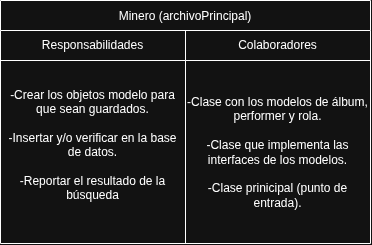
\includegraphics[width=0.5\textwidth]{CrcMinero.png}
  \caption{Responsabilidades del Minero.}
  \label{fig:fig1}
\end{figure}

\newpage
Con la figura anterior podemos describir brevemente y grandes rasgos el algoritmo que realiza el minero, al querer recorrer directorios y extraer metadatos, siguiendo el patrón de diseño DAO, cuando se le envía una ruta a este, el primer paso es hacer una verificación para comprobar que el directorio realmente exista; ya que, de lo contrario, avisa con un mensaje y se detiene para evitar errores. Si la ruta es válida, comienza a recorrer el directorio con el objetivo de encontrar únicamente los archivos con extensión .mp3, controlando posibles errores de permisos en las carpetas para que el programa no se caiga de la nada. Con los datos obtenidos de las etiquetas ID3v2.4.0 se construyen los objetos de los modelos y en caso de que llegue a faltar un dato como el título, se le coloca el nombre del archivo, o el nombre del directorio en el caso del álbum, o también ``Desconocido'' en el caso del no poder leer este valor y/o no tener performer. Para insertar; primero se busca el álbum y el performer para recuperar sus id y evitar duplicados, y ya con esos dos id termina de armar y guardar la rola.

Y al terminar de minar el directorio el minero reporta los id que se generan y de cada rola muestra el id que tiene como rola y el id que tiene al álbum que pertenece, de la misma forma con los performers y álbums muestra su nombre e id.


\newpage
\subsection*{Diseño de la Interfaz Gráfica}
Para el diseño de la interfaz gráfica, apoyándome en lo anterior dado por el análisis, el minero se puede y debe reutilizar completamente para que la vista sepa que dibujar en cuestion de resultados del minero, llegando a que uno se dedica únicamente a escanear carpetas y llenar SQLite, la interfaz se encarga de leer esa misma base de datos, presentarla de forma ordenada y permitirle al usuario interactuar con ella sin tocar la consola.

Decidí dividir la vista en varias clases para que no quedara todo amontonado (aunque creo que al final si se fue mucho a la clase principal de la vista): primero una clase encargada de iniciar y verificar que el archivo de lectura/guardado exista, otra clase dedicada a crear y usar al minero para poder elegir carpetas y que haga la búsqueda exclusivamente, avisando cuando termine para que la vista pricipal se actualice sola al terminar, también otra clase que se encargue de ``representar'' las filas de cada rola para que sean dibujados de forma más sencilla y por último la clase que contiene toda la lógica que se dedica a armar las columnas, hacer las consultas y filtros en segundo plano, abrir las ventanas secundarias para editar canciones o registrar personas y bandas, además de sacar la carátula y controlar el reproductor de audio; todo esto unido y que se arma cada vez en la clase que actua como punto de entrada de la interfaz gráfica.


\begin{figure}[htbp]
  \centering
  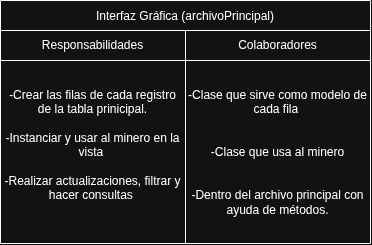
\includegraphics[width=0.5\textwidth]{CrcInterfaz.png}
  \caption{Responsabilidades del cliente.}
  \label{fig:fig2}
\end{figure}

Para describir brevemente el algoritmo de la interfaz gráfica, resulta en algo menos complejo (hasta cierto punto) ya que no se recorren directorios, sino que se usa lo que el usario haga, ya que por si sola no haría nada. Al iniciar por primera vez revisa y que exista el archivo donde va a leer sus datos o modificarlos y lo crea, para la segunda vez que inicie solo verifica que siga existiendo. Si el usuario decide buscar música, esto se hace en un ``segundo plano'' para evitar congelar la pantalla, al terminar el minero avisa a la vista que terminó para que actualice el contenido de la tabla principal. Dependiendo de lo que el usuario quiera, puede hacer búsquedas que filtran por título de rola, álbum, género o performer (solo uno a la vez), esto realiza una consulta dentro de la base de datos y le indica a la vista que mostrar dependiendo del resultado. Para editar los datos de una canción implica en hacer una actualización en la base de datos, ejecutando las operaciones de SQLite siempre en segundo plano para no provocar que se cuelge la aplicación.

Además, si el usuario selecciona una fila, el programa busca la ruta del .mp3 para extraer y mostrar su carátula; y si le da doble clic, carga el archivo en el reproductor de la interfaz para reproducirlo mientras un temporizador va actualizando la barra de progreso y el tiempo.

En sí tanto la vista como el minero trabajan sobre el mismo archivo .db pero muy separados para que este último se pueda ejecutar solo desde la terminal sin depender de la interfaz.

\newpage
\section{Implementación}
La implementación del proyecto decidí hacerlo nuevamente en C\# debido a que ya he trabajo en este lenguaje para el proyecto anterior, y siento conocer mejor como funciona 

Siguiendo el mismo detalle de que al compilarlo deja como un ejecutable un .exe, lo cual pues no me gusta y seguí utilizando la forma de compilar conocida como:``NativeAOT'' o en sus siglas en inglés ``Ahead-of-Time'' que como dice su nombre permite compilar el código directamente a código de maquina nativo, en lugar de su compilación habiatual. Un detalle es que una de sus limitaciones es que elimina algo llamado ``Reflexión'', es decir, no se puede generar código en tiempo de ejecución y fue una cosa que en un inicio no le di mucha importancia. Además de que en un punto al usar ciertas bibliotecas son completamente incompatibles con esta forma de compilar.

Para poder empezar a implementar primero el servidor, El lenguaje ya cuenta con la biblioteca System.IO que permite con Directory.EnumerateFiles y con SearchOption.AllDirectories recorrer facilmente los directorios de manera recursiva, y que se fije solamente en los .mp3 para que con ayuda de otra biblioteca llamada TagLibSharp se pueda extraer los datos de la etiqueta ID3v2.4.0 y meterlos a la base de datos con ayuda de SQLite, que en este lenguaje se puede hacer mediante la biblioteca Microsoft.Data.Sqlite. Investigando vi que permite hacer sus operaciones de manera ``Parametrizadas'' algo así como ``(@path), (@name)'' de esta forma se evita que ocurran errores con carácteres desconocidos y también evita inyecciones SQL.

En el punto de entrada desde la terminal es MineroBDD, el cual primero manda a llamar a IniciaBDD.Inicia() para verificar si el archivo rolas.db (que es donde ocurre el guardado, consultas, etc) en el directorio XDG de linux, especificamente en ~/.local/share mediante Environment.SpecialFolder.LocalApplicationData, sino lo encuentra lo crea con las tablas de .sql.

A partir de ahí, se instancian las clases concretas que implementan las interfaces de Interfaz.cs (Album, Performer y Rola) y se le pasan por constructor a la clase Minero, cada una tiene su metodo de insertar a la base de datos como: insertaBusca, insertaBuscaP e insertaBuscaR) que primero hace un SELECT para revisar si el registro ya existe y, si no está, hace el INSERT junto con SELECT last insert rowid()   para devolver el id recién generado y que el minero pueda ligar las llaves foráneas correctamente.

En este punto fue donde noté el detalle de usar AOT y era que el minero no lograba leer los archivos .mp3 correctamente aunque el código estuviera bien, daba errores similares a que el constructor de la clase TagLibSharp no estaba definido fuera de la clase y es que como mecioné al inicio esta biblioteca igual usa mucho la Reflexión para decidir que tipo de archivo de audio va a leer y el compilador con este modo es muy agresivo y cree que ese código no será utilizado y por ende lo borra para reducir tamaño del ejecutable. Para solucionarlo tuve que agregar una linea que es similar a ``DynamicDependency'' arriba del método principal del Minero y lo que hace es decirle al compilar que no le borre nada a la biblioteca y se conserve en tiempo de ejecución sin problemas.

También agregué bloques try-catch para que si ocurre algún problema con los .mp3 como no tener permisos de lectura de un directorio o que el archivo no tenga el formato correcto de la etiqueta, se avisan sin detener todo el proceso del minero.

\newpage
Para la implementación de la interfaz gráfica utilicé la biblioteca de GTK4 en C#. El primer paso fue crear la ventana principal en BDDMusicalV usando Application.New y su evento OnActivate, donde se inicializa la base de datos y se acomodan los dos componentes principales: VistaMinero arriba y VistaTabla en el centro, conectados mediante una acción de terminar para que en cuanto el minero acabe de buscar, la tabla se recargue sola.

En VistaMinero, pude encontrar la forma de utilizar el cuadro de dialogo que abre el explorador del sistema para seleccionar el directorio para buscar, esto mediante FileDialog con SelectFolderAsync. Y para evitar que la interfaz se congelara mientras se escanean muchos archivos, la ejecución del minero se delega a un hilo secundario usando Task.Run, desactivando temporalmente los botones mientras trabaja (aunque en la práctica esto no se nota mucho porque es algo muy rápido), y también si se intenta modificar elementos visuales con otro hilo, es decir que choquen se puede congelar la interfaz, por lo tanto los mensajes que regresa el minero se mandan a la etiqueta de estado envolviéndolos en GLib.Functions.IdleAdd, asegurando que la interfaz se actualice de forma segura en el hilo principal.

Para dibujar los datos en VistaTabla usé el ColumnView conectado a un Gio.ListStore y un SingleSelection para que ListStore pueda guardar las filas, la clase FilaTabla tuvo que declararse como partial y con el atributo [Subclass<GObject.Object>], de modo que GTK la reconozca como un objeto nativo y funcionaba sin problemas, ya que sin esto tenía problemas de compilación y está era la unica forma de arreglarlo, aunado a que al tratar de compilarlo con AOT daba muchisimos problemas de compilación y solución fue quitar esta forma por otra llamada ``PublishSingleFile'' algo similar al anterior pero que no recorta la reflexión del programa. Todas las consultas pesadas a SQLite como LlenarTabla, el filtrado en tiempo real como en Filtrar, la edición en ActualizarC y el registro de personas, bandas y uniones a grupos también se ejecutan dentro de Task.Run para mantener la ventana fluida y que no se caiga el programa.

Aprovechando la ruta física de cada canción guardada en la base de datos (que de hecho se pide para guardarla en la misma), se implementaron dos métodos extra en VistaTabla al seleccionar una fila con OnSelectionChanged, el método VerCaratula extrae la imagen incrustada del .mp3 con la biblioteca de TagLibSharp y la guarda temporalmente en /tmp/caratula bddmusical.jpg y la muestra mediante Gtk Picture, e igual usando el motor de gtk al dar doble click permite usar la ruta del .mp3 para que se ejecute con Gtk.MediaFile y activa la reproducción de la misma, agregando el temporizador con GLib.Functions.TimeoutAdd para que mueva la barra de reproducción cada 500 milisegundos.

\newpage
\section{Conclusión}
Al hacer este proyecto igual desde cero aplicando el modelo de la cascada cambia algo, ya que se puede planear la forma del algoritmo pero es diferente a la hora de implementar y puede encontrarse topes como el AOT que recorta demasiado a las bibliotecas que no están pensadas para compilarse de esta forma, lo cual, causa que se cambien cosas que no se tienen planeadas, vaya.

Con este proyecto en la parte de la interfaz gráfica, siento que comprendí de mejor forma los temas de ICC sobre los hilos de ejecución se relacionan con las interfaces para evitar que se cuelgen y como sincronizarlosm ya que en el proyecto anterior no hice eso por como los diccionarios lo hacian internamente.


\subsection{Bibliografia}
ORACLE. Design patterns: Data access object. (s. f.). https://www-oracle-com.translate.goog/java/technologies/data-access-object.html?_x_tr_sl=en&_x_tr_tl=es&_x_tr_hl=es&_x_tr_pto=tc

LakshanF. (s. f.). Create a single file for application deployment - .NET. Microsoft Learn. https://learn.microsoft.com/en-us/dotnet/core/deploying/single-file/overview?tabs=cli

Ajcvickers. (s. f.). Información general - Microsoft.Data.Sqlite. Microsoft Learn. https://learn.microsoft.com/es-es/dotnet/standard/data/sqlite/?tabs=net-cli

Microsoft. (s.f.). Implementación de AOT nativo. Microsoft Learn.  de https://learn.microsoft.com/es-es/dotnet/core/deploying/native-aot/

Gurovich, EV (2012). Introducción a las Ciencias de la Computación con JAVA. Universidad Nacional Autónoma de México. Facultad de Ciencias
\end{document}
